%\section*{Wavefunction and Schr$\ddot{o}$dinger equation}
%%%%%%%%%%%%%%%%%%%%%%%%%%%%%%%%%%%%%%%%%%
\begin{frame}
    \frametitle{}
    \begin{center}
    { {\huge Chapter-II Wavefunction and Schr$\ddot{o}$dinger equation }}
    \end{center}    
\end{frame}
%%%%%%%%%%%%%%%%%%%%%%%%%%%%%%%%%%%%%

\subsection{Wavefunction assumption}

\begin{frame}
    \frametitle{Review}
    \begin{center}
        Wave-particle duality is the inherent attribute of matter \\
        ~~\\
        ~~\\
        That brings big problems in interpret the reality world! \\
    \end{center} 
\end{frame}

\begin{frame}
    \frametitle{Two-slit experiments}
    \begin{center}
        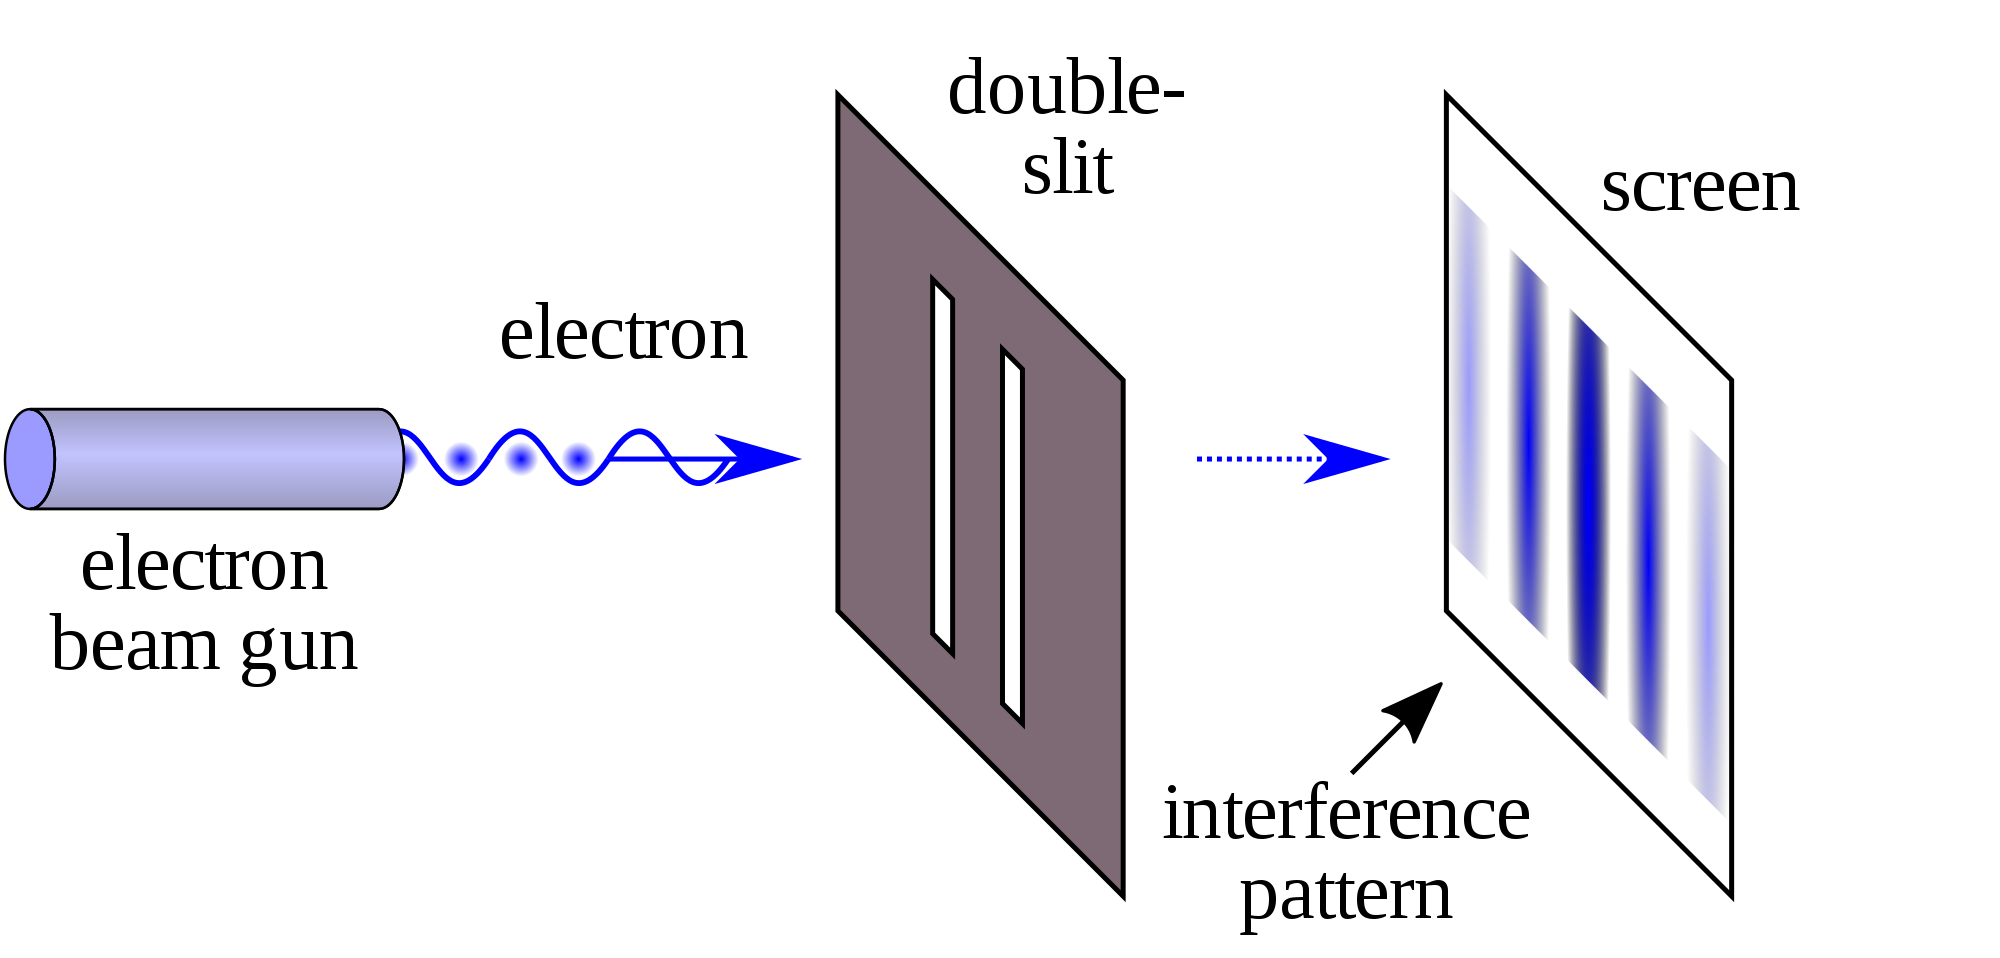
\includegraphics[width=0.8\textwidth]{figs/Etwoslitexp.png} \\
        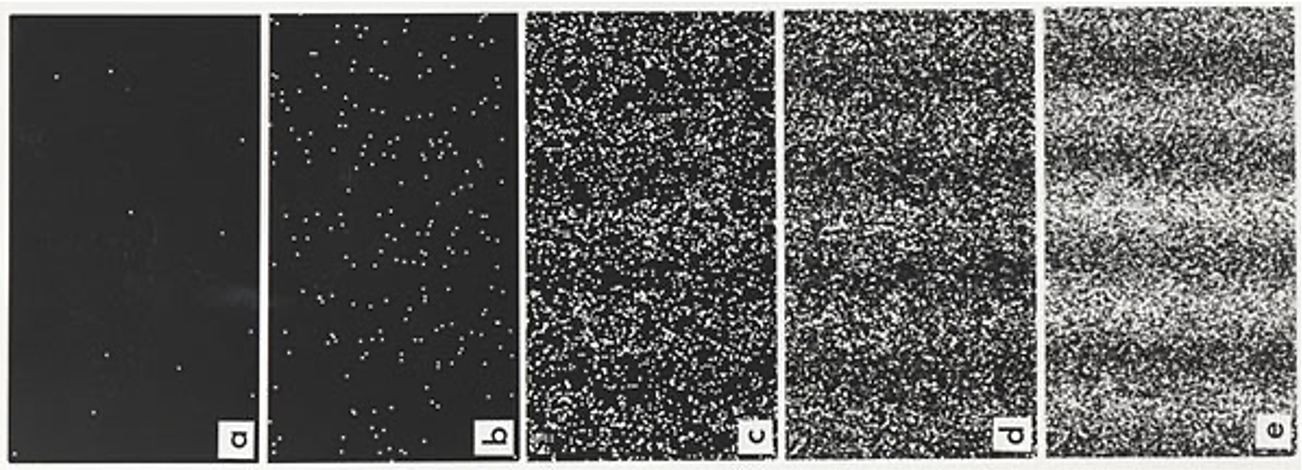
\includegraphics[width=0.7\textwidth]{figs/two-slit.png} \\
    \end{center} 
\end{frame}

\begin{frame}
    In 1924, De Broglie assumes that:\\
    \begin{tcolorbox}[colback=yellow!10,colframe=red!75!black,title=Basic assumption 1/5]
    The state of a system is described by a wavefunction
    \end{tcolorbox}
\end{frame}

\begin{frame}
    \frametitle{Constructing a quantum plane wave}
        For the classical plane wave
        \begin{equation*}
            \begin{split}
                y(x,t)&=A e^{i(\frac{2\pi}{\lambda}x-\omega t)} \\
                    & = A e^{i\frac{2\pi}{h}(\frac{h}{\lambda}x-h\nu t)}
            \end{split} 
        \end{equation*}
        For a free particle, put the De Broglie relationship into the formula, we get a quantum plane wave
        \begin{equation*}
            \begin{split}
                \Psi_p(x,t)&=A e^{\frac{i}{\hbar}(px-Et)}
            \end{split} 
         \end{equation*}
         For general wavefunction, it should be a wave-packet of plane wave
         \begin{equation*}
                \Psi(x,t)=\sum\limits_{p=0} ^{\infty} c(p)\Psi_p(x,t) = \int\limits_{p=0} ^{\infty} c(p,t) e^{\frac{i}{\hbar}px}dp
         \end{equation*}
\end{frame}

%%%%%%%%%%%%%%%%%%%%%%%%%%%%%%%%%
\subsection{Born's statistical interpretation}

\begin{frame}
    In 1926, Born proposed the statistical interpretation of the wavefunction
    \begin{tcolorbox}[colback=yellow!10,colframe=red!75!black,title=]
        The magnitude of the wave function $\Psi(\vec{r},t)$ does not tell us how much of 
        the particle is at position $\vec{r}$ at time t, 
        but rather the probability (W) that the particle is at or near the position at time t. \\
        \[ d W = |\Psi(\vec{r},t)|^2 d \tau \]
    \end{tcolorbox}
    {\color{deepred} Nobel Prize in physics(1954)}
\end{frame}

\begin{frame}[allowframebreaks=]
    \frametitle{Mathematical description}
    \begin{enumerate}
        \item Magnitude of the wave function \[|\Psi|^2 =\Psi^* \Psi \]
        \item Probability density \[\omega = |\Psi|^2 \]
        \item Probability  \[ d W = |\Psi|^2 d \tau \]
        \item Normalization \[ \int_{\Omega} |\Psi|^2 d \tau =1 \]
        \item Momentum wave-function \[ c(\vec{p},t)=\frac{1}{(2\pi\hbar)^{3/2}} \int_{0}^{\infty} \Psi(\vec{r},t) e^{\frac{-i}{\hbar} \vec{p}\cdot \vec{r} } d \tau \] 
        \item Expectation value of any function $f (x)$  \[ <f(x)>=\int_{0}^{\infty} f(x) |\Psi(x)|^2 dx \]
        \item Expectation value of observable A \[ <A>=\int_{0}^{\infty} \Psi^*(x) [A \Psi](x)| dx \]
    \end{enumerate}
\end{frame}

\begin{frame}
    \frametitle{Tips}
    \bullet $\Psi$ and $C\Psi$ describe the same state 
    \[ \frac{C\Psi(x_1)}{C\Psi(X_2)} = \frac{\Psi(x_1)}{\Psi(X_2)}\]
    \bullet $\Psi$ and $e^{i\varpi}\Psi$ describe the same state 
    \[ |e^{i\varpi}\Psi|^2 = e^{-i\varpi} e^{i\varpi} |\Psi|^2 = |\Psi|^2 \]   
\end{frame}

\begin{frame}
    \frametitle{Tips}
    Statistical interpretation requires wavefunction $\Psi$ to be:
    \bullet monotropic function\\
    \bullet continuous function \\
    \bullet finite function\\
    \bullet square integrable function
\end{frame}

\begin{frame}[allowframebreaks=]
    \frametitle{Appendix}
    \bullet 1. Normalizating the wavefunction \[\psi(x)=\sin(x), \qquad (0\le x \le \pi)\]
    \alert{Solve:} assuming the normalized wavefunction 
    \[\Psi=C\sin(x)\]
    \begin{equation*}
        \begin{split}
            \int_0 ^\pi |C\sin(x)|^2 dx &=1 \\
            C^2 \int_0 ^\pi \sin^2(x) dx &=1 \\
            C^2 \int_0 ^\pi \frac{1-\cos 2x }{2} dx &=1 \\ 
            C^2 [\frac{x}{2}-\frac{\sin 2x}{4}]_0 ^\pi &=1 \\ 
        \end{split} 
     \end{equation*}
     \[C=\sqrt{\frac{2}{\pi}}\]
     The normalized wavefunction:
     \begin{equation*}
        \Psi=C\sin(x)=\sqrt{\frac{2}{\pi}}\sin(x)
    \end{equation*}
    \bullet 2. Normalizating the plane wave \[\Psi_p (x,t)=e^{\frac{i}{\hbar}(px-Et)} \] 
    \alert{Solve:} it's not a square integrable function, assuming the normalized wavefunction 
    \[\Psi=C\Psi_p (x,t)\]
    \begin{equation*}
        \begin{split}
            \int_{-\infty} ^\infty |C\Psi_p (x,t)|^2 dx &=1  \\
            C^2 \int_0 ^\infty \Psi_p (x) \Psi_{p'} (x) dx &=\delta (p-p')  \\
            C^2 \int_0 ^\infty e^{\frac{i}{\hbar}(p-p')x} =&=\delta (p-p')\\
            C^2 2\pi \hbar \delta (p-p') &=\delta(p-p') \\
            C&= \frac{1}{\sqrt{2\pi \hbar}}
        \end{split} 
     \end{equation*}
     The normalized wavefunction:
     \begin{equation*}
        \Psi=\frac{1}{\sqrt{2\pi \hbar}} e^{\frac{i}{\hbar}px}
    \end{equation*}  
\end{frame}

%%%%%%%%%%%%%%%%%%%%%%%%%%%%%%%%%
\subsection{Superposition principle of states}
%%%%%%%%%%%%%%%%%%%%%%%%%%%%%%%%%%
\begin{frame}
    \frametitle{Superposition principle of states}
    \begin{tcolorbox}[colback=yellow!10,colframe=red!75!black,title=]
    Born also proposed that \\
    \bullet if $\psi_1$ and $\psi_2$ are the possible states of the system,
    their linear superposition \[ \Psi=c_1 \psi_1+ c_2\psi_2 \]
    is also the possible state of the system.\\
    \bullet if the system locates at the superposition $\Psi$, the possiblity of observating the system at $\psi_i$ is $|c_i|^2$, and 
    \[\sum_i |c_i|^2 =1\]
    \end{tcolorbox}
\end{frame}

\begin{frame}
    \begin{corollary}
    If we know eah eigenstate $\{ \psi_1,\psi_2,\cdots,\psi_n \}$ of an observable A, 
    any possible states of the system can be described as \[ \Psi=c_1 \psi_1+ c_2\psi_2+\cdots+c_n\psi_n\] 
    \end{corollary}
    Hence, we have :
    \begin{equation*}
        \Psi(x,t)=\sum\limits_{p=0} ^{\infty} b(p)\Psi_p(x,t) = \int\limits_{p=0} ^{\infty} c(p,t) e^{\frac{i}{\hbar}px}dp
    \end{equation*}
    \[ c(\vec{p},t)=\frac{1}{(2\pi\hbar)^{3/2}} \int_{0}^{\infty} \Psi(\vec{r},t) e^{\frac{-i}{\hbar} \vec{p}\cdot \vec{r} } d \tau \] 
\end{frame}

\begin{frame}
    Explanation of the two-slit experiment.\\
    ~~\\
    \bullet Lets $\psi_1$ describe the state of the electron run across slit-1 and $\psi_2$ for slit-2. \\
    \bullet when both of them are opened, the electron locates the superposition 
    \[ \Psi=c_1 \psi_1+ c_2\psi_2 \]
    \bullet the possiblity of electron reaches each point of screen 
    \begin{equation*}
        \begin{split}
            |\Psi|^2 &= (c_1 \psi_1+ c_2\psi_2)^* (c_1 \psi_1+ c_2\psi_2) \\
            & = |c_1|^2 |\psi_1|^2 + |c_2|^2 |\psi_2|^2  + [c_1 c_2 ^* \psi_1 \psi_2 ^* + c_1 ^* c_2 \psi_1 ^* \psi_2] \\
        \end{split} 
     \end{equation*}
     \bullet the interference pattern comes from  
     \[[c_1 C_c ^* \psi_1 \psi_2 ^* + c_1 ^* c_2 \psi_1 ^* \psi_2] \]
\end{frame}

\begin{frame}
    \frametitle{Which way?}
    The probabilistic interpretation was controversial from the beginning of of quantum mechanics
    \begin{itemize}
        \item De Broglie : Pilot waves
        \item Schr$\ddot{o}$dinger: Schr$\ddot{o}$dinger's cat
        \item Einstein: EPR paradox
        \item Wheeler's delayed choice experiment
        \item Quantum eraser experiment
        \item $\cdots \cdots$
    \end{itemize}
\end{frame}

\begin{frame}
    \frametitle{Schr$\ddot{o}$dinger's cat}
    \begin{center}
        \includegraphics[width=0.8\textwidth]{figs/cat.jpeg} \\
    \end{center} 
\end{frame}

\begin{frame}
    \frametitle{EPR paradox}
    \begin{center}
        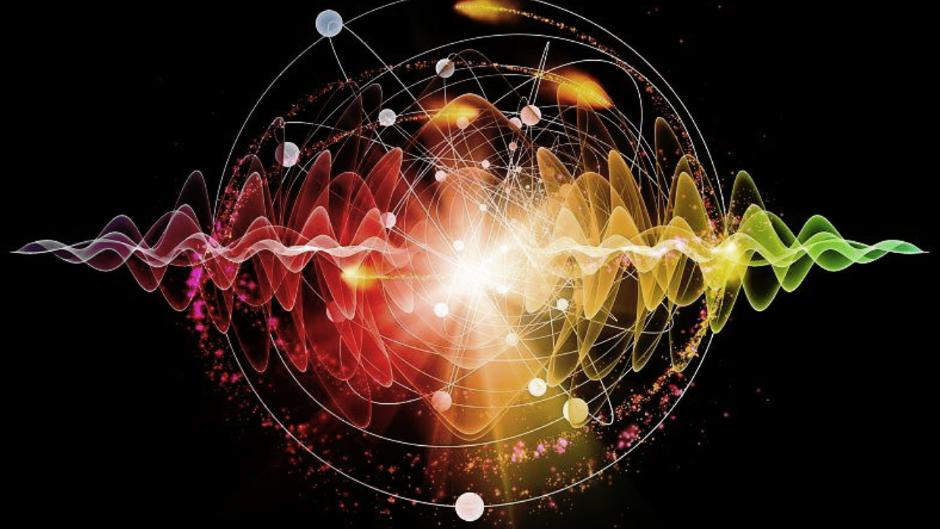
\includegraphics[width=1.0\textwidth]{figs/EPR.jpeg} \\
    \end{center} 
\end{frame}

\begin{frame}
    \frametitle{The bell inequality}
    \begin{center}
        \includegraphics[width=1.0\textwidth]{figs/bell.png} \\
    \end{center} 
\end{frame}

\begin{frame}
    \frametitle{Wheeler's delayed choice experiment}
    \begin{center}
        \includegraphics[width=0.8\textwidth]{figs/choose.png} \\
    \end{center} 
\end{frame}

\begin{frame}
    \frametitle{Quantum eraser experiment}
    \begin{center}
        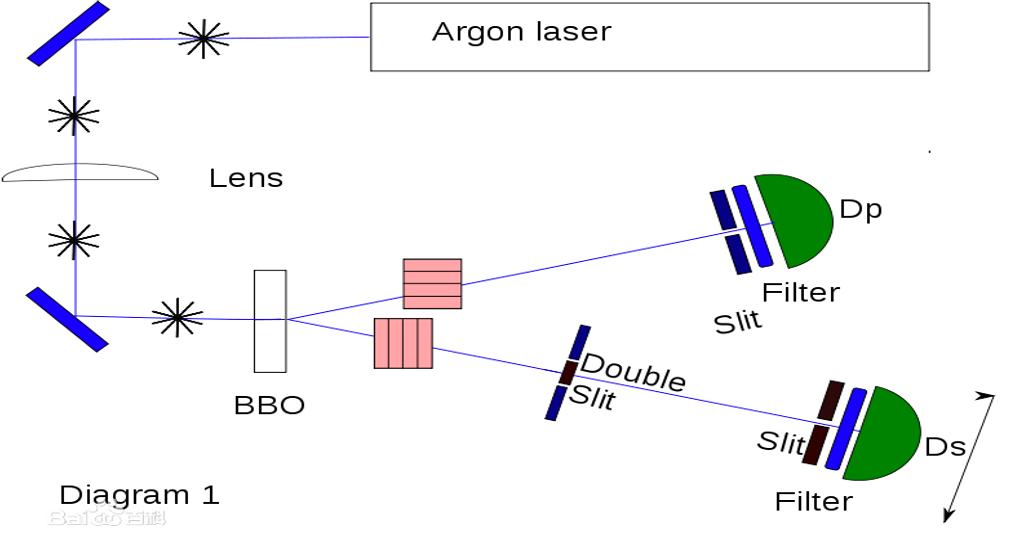
\includegraphics[width=1.0\textwidth]{figs/chachuexp.png} \\
    \end{center} 
\end{frame}

\begin{frame}
    \frametitle{}
    \begin{center}
        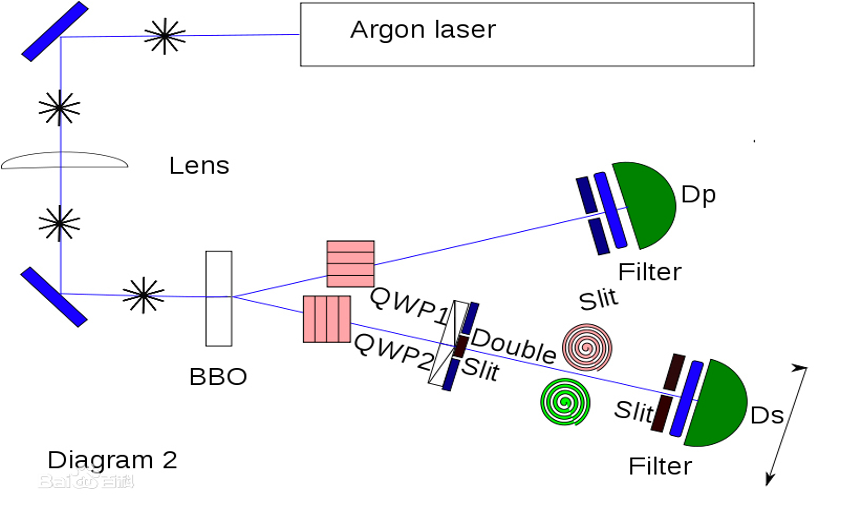
\includegraphics[width=1.0\textwidth]{figs/chachuexp_2.png} \\
    \end{center} 
\end{frame}

\begin{frame}
    \frametitle{}
    \begin{center}
        \includegraphics[width=1.0\textwidth]{figs/chachuexp_3.png} \\
    \end{center} 
\end{frame}

\begin{frame}
    \frametitle{Summary}
    \begin{enumerate}
        \item Objects are wave-particles and can be in states of superposition
        \item Measurement changes the states and gives random results
        \item Measurement results are complementary
        \item Measurement leads to objective reality
    \end{enumerate}
\end{frame}

%%%%%%%%%%%%%%%%%%%%%%%%%%%%%%%%%
\subsection{Schr$\ddot{o}$dinger equation}
%%%%%%%%%%%%%%%%%%%%%%%%%%%%%%%%%%
\begin{frame}
    \begin{tcolorbox}[colback=yellow!10,colframe=red!75!black,title=Basic assumption 2/5]
        The evolution of wavefunction obeys Schr$\ddot{o}$dinger equation
        \begin{equation*}
            i\hbar \frac{\partial }{\partial t} \Psi (\overrightarrow{r},t ) =\left [ -\frac{\hbar^2}{2\mu }\nabla ^2 + V(\overrightarrow{r},t ) \right ]\Psi (\overrightarrow{r}, t ) 
        \end{equation*}
    \end{tcolorbox}
\end{frame}

\begin{frame}
    \frametitle{Constructing Schr$\ddot{o}$dinger equation}
    \bullet Plane wave-function ($\psi(x,t)=\Psi_p(x,t)=e^{\frac{i}{\hbar}(p\cdot x-Et)}$) be a sulotion of Schr$\ddot{o}$dinger equation, obviously
    \begin{equation*}
        \begin{split}
       -i\hbar \nabla \psi(x,t) &=p\psi(x,t) \\
       \hbar^2 \nabla^2 \psi(x,t) &=p^2\psi(x,t) \\
       \frac{\hbar^2}{2\mu} \nabla^2 \psi(x,t) &=\frac{p^2}{2\mu} \psi(x,t) , \qquad \cdots (1)
        \end{split}
    \end{equation*}
    \begin{equation*}
       i\hbar \frac{\partial }{\partial t} \psi(x,t) =E\psi(x,t)  , \qquad \cdots (1)
     \end{equation*}
    (2)-(1)
    \begin{equation*}
        (i\hbar \frac{\partial }{\partial t} - \frac{\hbar^2}{2\mu} \nabla^2 )\psi(x,t) =(E-\frac{p^2}{2\mu})\psi(x,t)=0  
    \end{equation*}
\end{frame}

\begin{frame}[allowframebreaks=]
    \begin{equation*}
        i\hbar \frac{\partial }{\partial t} \psi(x,t) = \frac{\hbar^2}{2\mu} \nabla^2 \psi(x,t)
    \end{equation*}
    For general wavefunction, it's a wave packet of plane wave
    \begin{equation*}
        \Psi(x,t)= \int\limits_{p=0} ^{\infty} c(p,t) e^{\frac{i}{\hbar}px}dp
    \end{equation*}
    we get 
    \begin{equation*}
        \begin{split}
        (i\hbar \frac{\partial }{\partial t} - \frac{\hbar^2}{2\mu} \nabla^2 )\Psi(x,t) &= \int\limits_{p=0} ^{\infty} c(p,t) (E-\frac{p^2}{2\mu}) e^{\frac{i}{\hbar}px}dp=0  \\
        i\hbar \frac{\partial }{\partial t} \Psi(x,t) &= \frac{\hbar^2}{2\mu} \nabla^2 \Psi(x,t)
        \end{split}
    \end{equation*}
    For nonfree particle in a potential $U(x)$,
    \begin{equation*}
        i\hbar \frac{\partial }{\partial t} \Psi(x,t) = (\frac{\hbar^2}{2\mu} \nabla^2 +U(x)) \Psi(x,t)
    \end{equation*}
    That is the Schr$\ddot{o}$dinger equation. \\
    ~~\\
    \bullet For N-particles system
   {\small \begin{equation*}
        i\hbar \frac{\partial }{\partial t} \Psi(x_1, x_2, \cdots x_N,t) = [\sum_{i=1} ^{N} \frac{\hbar ^2}{2\mu_i} \nabla^2 +U(x_1, x_2, \cdots x_N)] \Psi(x_1, x_2, \cdots x_N,t)
    \end{equation*}}
\end{frame}

\begin{frame}

\end{frame}

\begin{frame}
\end{frame}

\begin{frame}
\end{frame}

\begin{frame}
\end{frame}

\begin{frame}
\end{frame}

\begin{frame}
\end{frame}

